\chapter{SVD used for compression of FEA results}
\label{chapter:SVD}

Singular Value Decomposition (SVD) is a well known factorization method that provides rich information about matrix systems \cite{Baker2005, Kalman1996, Golub1996, Duintjer2012}. One of its many applications is image compression where it can significantly reduce size of data representing image while preserving quality of image appearance. Considering the fact that the results from FEM analyses can be viewed as a series of arbitrary rectangular matrices, the implementation of compression algorithm based on SVD is straightforward as it can be applied to any rectangular matrix. This chapter contains the description of the compression method based on SVD that is the key part of the storage format proposed in this thesis. The content of this chapter is also published in \cite{Benes2018}.

%----------------------------------------------------------------------------------------
%	SECTION Mathematical background
%----------------------------------------------------------------------------------------

\section{Mathematical background}

Singular value decomposition is based on a theorem from linear algebra which says that a rectangular matrix $\mtrx{A} \in \mathbb{R}^{m \times n}$ can be decomposed into the product of three matrices - an orthogonal matrix $\mtrx{U} \in \mathbb{R}^{m \times m}$, a diagonal
matrix $\mtrx{S} \in \mathbb{R}^{m \times n}$, and the transpose of an orthogonal matrix $\mtrx{V} \in \mathbb{R}^{n \times n}$:

\begin{equation}
\mtrx{A} = \mtrx{U} \mtrx{S} \mtrx{V}^\mathsf{T},
\label{eq:svd-def}
\end{equation}

\noindent
where $\mtrx{U^\mathsf{T}U} = \mtrx{I}$, $\mtrx{V^\mathsf{T}V} = \mtrx{I}$. The columns of $\mtrx{U}$ are orthonormal eigenvectors of $\mtrx{AA^\mathsf{T}}$, which are called the left singular vectors. The columns of $\mtrx{V}$ are orthonormal eigenvectors of $\mtrx{A^\mathsf{T}A}$ called the right singular vectors. $\mtrx{S}$ (sometimes referred to as $\mtrx{\Sigma}$) is a diagonal matrix containing singular values in descending order, which are at the same time the nonzero square roots of the eigenvalues of $\mtrx{AA^\mathsf{T}}$ and $\mtrx{A^\mathsf{T}A}$.

SVD can be seen as a method for transforming correlated variables into a set of uncorrelated ones. At the same time, SVD is a method for ordering the dimensions based on variation and identifying the dimension with the largest variation. Once this dimension is identified, it is possible to find the best approximation of the original data points using fewer dimensions. Hence, SVD can be seen as a method for data reduction/compression.

\subsection{SVD compression}

This is the basic idea behind SVD: taking a high dimensional, highly variable set of data points and reducing it to a lower dimensional space that exposes the substructure of the original data more clearly and orders it from the largest variation to the least. What makes SVD practical for data compression applications is that variation below a particular threshold can be simply ignored to massively reduce data with assurance that the main relationships of interest have been preserved.

The objective of a compression algorithm is to reduce amount of data representing FEM results and also the ability to reconstruct original data from its smaller representation. This saves storage capacity and also accelerates the data transfer between computers as the analysis itself and the post-processing of results is sometimes done on different workstations.

A compression method can be lossy or lossless. Lossless methods are able to fully reconstruct original data. Lossy methods, on the other hand, produce only approximations of original data.

SVD is used in this thesis as a part of the compression algorithm. The SVD method applied to arbitrary matrix produces decomposition that consists of corresponding singular values and singular vectors. This process is fully reversible (with the assumption that the numerical errors are negligible). The original matrix can be reconstructed by the multiplication of decomposed parts. However, the compression algorithm is based on modification of decomposition to create low-rank approximation matrix. The reconstructed matrix slightly differs from the original matrix and algorithm therefore performs lossy compression.

\subsection{Low-rank approximation matrix}

From the definition of SVD in (\ref{eq:svd-def}) and from the properties of SVD, the fact follows that a matrix can be represented in the form of its SVD components as a sum of $k$ rank-1 matrices

\begin{equation}
\mtrx{A}=\sum_{i=1}^{k} s_{i}\mathbf{u}_{i}\mathbf{v}_{i}^{\mathsf{T}},
\label{eq:svd-expansion}
\end{equation}

\noindent
where $s_i$ is the $i$-th singular value of matrix $\mtrx{A}$, $\mathbf{u}_i$ and $\mathbf{v}_i$ are corresponding singular vectors of matrix $\mtrx{A}$, and $k = \mathrm{min}(m, n)$. Considering the fact that singular values are ordered $s_{1} \geq s_{2} \geq s_{3} \geq ... \geq s_{k}$, the above formula implies that the first term of the sum would have the highest contribution and the last term would have the lowest contribution to matrix~$\mtrx{A}$. Therefore, if we take only first $r$ members of the above summation we get an approximation matrix

\begin{equation}
\mtrx{A'}=\sum_{i=1}^{r} s_{i}\mathbf{u}_{i}\mathbf{v}_{i}^{\mathsf{T}}.
\label{eq:svd-approx-expansion}
\end{equation}

Quality of approximation depends on the magnitude of the singular values omitted from the approximation formula, namely $s_{r+1} ...  s_{k}$. The compression algorithm is based on an assumption that the first singular value is order-of-magnitude higher than singular values at the end of the decomposition sequence. In special cases, when $r=k$, or $s_{i}=0$ for all $i > r$, the omitted singular values do not contribute to the sum and the compression is therefore lossless. In other cases, approximation error has to be calculated and taken into account to avoid loss of important details in data.

The main goal of the compression algorithm is to find a compromise between low approximation error and high compression ratio $c$ which is calculated using the formula

\begin{equation}
c=\frac{r(m+n+1)}{m n},
\label{eq:cr-def}
\end{equation}

\noindent
where $m$ is the number of rows and $n$ is the number of columns of matrix $\mtrx{A}$. Explanation of the compression ratio formula is best done using Figure~\ref{fig:lowrank_svd}. Light color represents the part of matrix decomposition that is to be stored in the output file as a low-rank approximation of the input.

\begin{figure}[H]
\centering
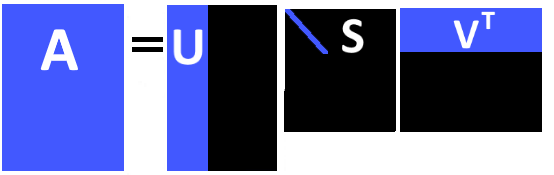
\includegraphics[width=0.7\textwidth]{figures/chapter-SVD/low_rank_decomposition_diagram}
\decoRule
\caption[Singular value decomposition illustration.]{Decomposition of input matrix $\mtrx{A}$ into diagonal matrix of singular values $\mtrx{S}$ and matrices of left and right singular vectors. Light color illustrates low-rank approximation.}
\label{fig:lowrank_svd}
\end{figure}

\subsection{Error estimation}
\label{sec:error-estimation}

Low-rank approximation matrix method, which was described above, is a lossy compression technique. Several error metrics are used to control the quality of results.

\begin{itemize}

\item \textbf{Mean Square Error}
\begin{equation}
\mathit{MSE}=\frac{1}{m n} \sum_{i=1}^{m} \sum_{j=1}^{n} (a_{ij} - a'_{ij})^{2},
\label{eq:mse-def}
\end{equation}

\noindent
where $a_{ij}$ represents an element of the original matrix and $a'_{ij}$ represents an element of the
reconstructed matrix of dimension $m \times n$.

\item \textbf{Rooted Mean Square Deviation}
\begin{equation}
\mathit{RMSD} = \sqrt{\mathit{MSE}}.
\label{eq:rmsd-def}
\end{equation}

\item \textbf{Normalized Rooted Mean Square Deviation}
\begin{equation}
\mathit{NRMSD} = \frac{\mathit{RMSD}}{X_{max}-X_{min}}=\frac{\sqrt{\mathit{MSE}}}{X_{max}-X_{min}},
\label{eq:nrmsd-def}
\end{equation}

\noindent
where $X_{min}$ and $X_{max}$ are elements of input matrix $\mtrx{A}$ with minimum and maximum value, respectively. This error metric is able to measure and compare errors in datasets with different scales. Therefore, it is the main parameter that is used to control the quality of compression in the proposed compression algorithm.

\item \textbf{Peak Signal to Noise Ratio}

$\mathit{PSNR}$ is most commonly used to measure the quality of reconstruction of lossy compression methods (e.g. image compression). The signal in this case is the original data, and the noise is the error introduced by compression. $\mathit{PSNR}$ is an approximation to human perception of reconstruction quality. This metric is not so important in area of FEM analyses, where the human perception of visualizations is not as important as the exact mathematical accuracy of approximations. The reason to include $\mathit{PSNR}$ in results is in particular to allow comparison with other image-related compression methods. $\mathit{PSNR}$ is usually expressed in terms of the logarithmic decibel scale (dB)

\begin{eqnarray}
\mathit{PSNR} &=& 10\log_{10}\frac{(X_{max}-X_{min})^{2}}{\mathit{MSE}} =
\\
&=& 20\log_{10}\frac{X_{max}-X_{min}}{\sqrt{\mathit{MSE}}}=20\log_{10}\frac{1}{\mathit{NRMSD}} = \nonumber
\\
&=& -20\log_{10}\mathit{NRMSD}. \nonumber
\label{eq:psnr-def}
\end{eqnarray}

\item \textbf{Normalized Maximum Error}
\begin{equation}
\mathit{NME} = \frac{\lVert \mtrx{A} - \mtrx{A'} \lVert_{\max}}{X_{max}-X_{min}} = \frac{\max\limits_{ij}(a_{ij} - a'_{ij})}{X_{max}-X_{min}}.
\label{eq:nme-def}
\end{equation}

\end{itemize}

\subsection{Randomized SVD}

There are many algorithms with different approaches to compute singular value decompositions. One approach is based on diagonalization of the matrix which essentially yields the whole decomposition at the same time. The other approach is the use of an iterative algorithm that yields one or several singular values at a time and can be stopped after desired number of singular values and vectors has been computed. Although these algorithms have proven to work very well for relatively small matrices, they are not well suited for using with large data sets. The exact SVD of a $m \times n$ matrix has computational complexity $\mathrm{O}(\mathrm{min}(mn^2, m^2n))$ using the ``big-O'' notation. When applied on large data sets it tends to be very time-consuming. Also, the modern hardware architectures use caches to optimize reading of consecutive memory blocks. As these algorithms often need random access to the memory where the input matrix is stored, it can increase communication between different levels in memory hierarchy, which causes higher latency when accessing data. From a numerical linear algebra perspective, an additional problem resulting from increasing matrix sizes is that noise in the data, and propagation of rounding errors, become increasingly problematic.

In \cite{Candes2011, Woolfe2008, Martinsson2011, Szlam2014}, there are described randomized methods for constructing approximate matrix factorizations which offer significant speedups over classical methods. The particular implementation of the randomized decomposition is based on the algorithm described in \cite{Halko2011}. The authors proposed an algorithm for efficient computation of low-rank approximation to a given matrix. The method uses random sampling to identify a subspace that captures most of the action of a matrix. The input matrix is compressed to this subspace, and deterministic manipulations are then used to obtain the desired low-rank factorization. For a matrix that is too large to fit in fast memory, the randomized techniques require only a constant number of passes over the data, as opposed to $\mathrm{O}(k)$ passes for classical algorithms.

The algorithm can be split into two main computational stages. The first stage is to construct a low-dimensional subspace that captures the action of the matrix. To be more formal, this stage is to compute an approximate basis for the range of the input matrix $\mtrx{A}$. This basis matrix $\mtrx{Q}$ is required to have orthonormal columns and

\begin{equation}
\mtrx{A} \approx \mtrx{Q} \mtrx{Q}^{\mathsf{T}} \mtrx{A}.
\end{equation}

\noindent
Matrix $\mtrx{Q}$ is desired to contain as few columns as possible while producing accurate approximation of matrix $\mtrx{A}$ at the same time.

The second stage is to use $\mtrx{Q}$ to obtain approximate SVD factorization of $\mtrx{A}$. This can be achieved using simple deterministic steps:

\begin{enumerate}
\item Construct $\mtrx{B} = \mtrx{Q}^{\mathsf{T}} \mtrx{A}$.
\item Compute an exact SVD of the small matrix: $\mtrx{B}=\mtrx{W}\mtrx{\widetilde{S}}\mtrx{\widetilde{V}}^{\mathsf{T}}$.
\item Set $\mtrx{\widetilde{U}}=\mtrx{Q}\mtrx{W}$.
\end{enumerate}

The main challenge is therefore to efficiently construct $r$ orthonormal vectors forming the matrix $\mtrx{Q}$ that (nearly) span the range of $\mtrx{A}$; $r$ is the desired rank of approximation and is supposed to be substantially less then both dimensions of $\mtrx{A}$. After that an SVD that closely approximates $\mtrx{A}$ can be constructed (closely in the sense that the spectral norm of the difference between $\mtrx{A}$ and the approximation to $\mtrx{A}$ is small relative to the spectral norm of $\mtrx{A}$).

In order to estimate the range of matrix $\mtrx{A}$, it is applied to a collection of $r$ random vectors. The result of applying $\mtrx{A}$ to any vector is a vector in the range of $\mtrx{A}$, and if the matrix is applied to $r$ random vectors, the results will nearly span the range of $\mtrx{A}$ with extremely high probability. Mathematical proofs given in \cite{Halko2011} and \cite{Witten2015} show that the probability of missing a substantial part of the range of $\mtrx{A}$ is negligible if the vectors to which matrix $\mtrx{A}$ is applied are sufficiently random (i.e. entries of these vectors are independent and identically distributed).

Therefore, matrix $\mtrx{A}$ is applied to a random Gaussian matrix $\mtrx{\Omega}$ that contains $r$ columns with random normally distributed entries yielding the matrix $\mtrx{Y} = \mtrx{A} \mtrx{\Omega}$. Applying the Gram-Schmidt process (or any other method for constructing QR decomposition) produces the decomposition $\mtrx{Y}=\mtrx{Q}\mtrx{R}$, where columns of $\mtrx{Q}$ are an orthonormal basis for the range of $\mtrx{Y}$, and since columns of $\mtrx{Y}$ nearly span the range of $\mtrx{A}$, $\mtrx{Q}$ is an orthonormal basis for the approximate range of $\mtrx{A}$.

$\mtrx{A}$ is then decomposed as
\begin{equation}
\mtrx{A} \approx \mtrx{Q}\mtrx{Q}^{\mathsf{T}}\mtrx{A} = \mtrx{Q}\mtrx{B} = \mtrx{Q}\mtrx{W}\mtrx{\widetilde{S}}\mtrx{\widetilde{V}}^{\mathsf{T}} = \mtrx{\widetilde{U}}\mtrx{\widetilde{S}}\mtrx{\widetilde{V}}^{\mathsf{T}}.
\end{equation}

\noindent
The algorithm produces matrices $\mtrx{\widetilde{U}}$ and $\mtrx{\widetilde{V}}$ with orthonormal columns being approximations of the left and the right singular vectors of matrix $\mtrx{A}$, and a nonnegative diagonal matrix $\mtrx{\widetilde{S}}$ that contains approximations of the first $r$ singular values of matrix $\mtrx{A}$. For a dense input matrix, randomized SVD algorithm requires $\mathrm{O}(mn \log{r})$ floating-point operations, substantially less than classical algorithms.


%----------------------------------------------------------------------------------------
%	SECTION Implementation
%----------------------------------------------------------------------------------------

\section{Implementation}

% SVD is applied on matrices. The first thing to do is therefore to assemble an input matrix. ...
% As an example, temperature field, vector of nodal displacements, strain tensor evaluated in integration points, etc. can serve. There are two similar sets of results. One is generated by a non-linear algorithms, where several incremental steps are stored and the other is generated by time integration, where results in particular time steps are stored. ...

Results from the finite element method are scalar, vector or tensor fields represented by discrete values calculated in nodes of the mesh or in integration points on finite elements. In order to compress data, an auxiliary matrix~$\mtrx{A}$ has to be assembled from the results. The number of rows of the matrix~$\mtrx{A}$ is equal to the number of incremental or time steps while the number of columns is equal to the number of points in which the results are stored. Such auxiliary matrix is assembled for each scalar field and for each component of the vector and tensor fields. It means, three matrices corresponding to the displacement in the $x$, $y$, and $z$ directions are assembled for the vector of displacements in three-dimensional problems.

There are two main reasons to store particular results in separate matrices. First, the size of matrices is smaller than the size of a matrix which contains all results and therefore SVD will be performed faster. Second, the magnitudes of particular fields are very different (the stress tensor components are several order of magnitude larger than the components of the displacement vector) and the data compression algorithm would suppress the fields with small magnitudes. Once the matrix $\mtrx{A}$ is assembled for each field, the compression algorithm can be applied on it. It is purely algebraic procedure and no information about geometry of the mesh is needed.

Let us assume that the matrix is not empty and is full rank. Then it follows from the formula (\ref{eq:cr-def}) that if $r$ is equal to the rank of matrix $\mtrx{A}$, the compression ratio is always higher than one. In other words the memory consumption of stored decomposition is bigger than the size of the original matrix. To make the compression algorithm applicable, the parameter $r$ must satisfy the condition

\begin{equation}
r<\frac{m n}{m+n+1}.
\label{eq:r-ineq}
\end{equation}

\noindent
Considering the usual shape of matrix containing FEM results, this inequality is easily satisfiable even for the $r$ being close to the rank of the original matrix as in the typical case the number of nodes or integration points is much higher than the number of analysis steps and therefore $m \ll n$.

\subsection{Algorithm description}
Once SVD is calculated, the compression algorithm removes a certain number of singular values and corresponding singular vectors. The remaining singular values and vectors represent the compressed data. There are two strategies that influence the way how to preserve the number of singular values -- resulting size and quality. Each strategy is assigned a control parameter that determines compression ratio or approximation error.

\paragraph{Compression ratio}
If the focus is only on the size of compressed data, the rank $r$ of the approximation matrix can be calculated by the formula

\begin{equation}
r=\ceil*{c \times \frac{m n}{m+n+1}},
\label{eq:rank-from-comp-ratio}
\end{equation}

\noindent
where $c$ is the compression ratio, $0 \leq c \leq 1$ ($0$ results in absolute compression while $1$ results in no compression); $\ceil*{.}$ is the ceiling function.

\paragraph{Approximation error}
In a usual case, the most important measure to take into account is the approximation error. Algorithm is trying to minimize the compression ratio while at the same time ensuring that predefined approximation error threshold is not exceeded. To quantify the error, the Normalized root-mean-square deviation ($\mathit{NRMSD}$) is used. The normalized error metric enables working with various data sets that have different scales. $\mathit{NRMSD}$ is defined in Section \ref{sec:error-estimation}.

To effectively calculate the final rank of the approximation matrix from the desired approximation error, the interesting property of singular values

\begin{equation}
\sum_{i=1}^{m} \sum_{j=1}^{n} (a_{ij})^{2} = \sum_{i=1}^{k}{s_{i}^{2}},
\label{eq:elem-sqr-sigma-sqr}
\end{equation}

\noindent
where $k=\mathrm{min}(m, n)$, i.e. the smallest of two dimensions of the matrix $\mtrx{A}$, is made use of. The above formula states that the sum of squared elements of the matrix $\mtrx{A}$ equals to the sum of squared singular values $s_{i}$ of the same matrix $\mtrx{A}$.

Using formulas \eqref{eq:svd-expansion} and \eqref{eq:svd-approx-expansion} the equation \eqref{eq:elem-sqr-sigma-sqr} can be applied to the difference between original matrix $\mtrx{A}$ and approximation matrix $\mtrx{A'}$

\begin{equation}
\sum_{i=1}^{m} \sum_{j=1}^{n} (a_{ij} - a'_{ij})^{2} = \sum_{i=r+1}^{k}{s_{i}^{2}},
\end{equation}

\noindent
where the term on the right-hand side is the sum of squares of those singular values of the matrix $\mtrx{A}$ that are going to be cut away by the compression algorithm. The equation can be rewritten using the definition of $\mathit{MSE}$ in \eqref{eq:mse-def} to

\begin{equation}
\mathit{MSE} \times m n = \sum_{i=r+1}^{k} s_{i}^{2}
\end{equation}

\noindent
and using \eqref{eq:nrmsd-def} further to

\begin{equation}
(\mathit{NRMSD} \times (X_{max}-X_{min}))^{2} \times m n = \sum_{i=r+1}^{k} s_{i}^{2}.
\end{equation}

Then $\mathit{NRMSD}$ can be used as a quality metric for the compression algorithm because normalization makes it usable for different datasets. Calculation of rank of the approximation matrix is depicted as pseudo-code in Algorithm \ref{alg:rank-calculation}. Algorithm uses the inequality

\begin{equation}
e > \frac{\sqrt[]{\frac{\sum_{i=r+1}^{k} s_{i}^{2}}{m n}}}{X_{max}-X_{min}}
\end{equation}

\noindent
to test whether the desired rank has been reached; $e$ is $\mathit{NRMSD}$ used as an error threshold that can not be exceeded to achieve desired quality of approximation.

\begin{algorithm}
  \caption{Calculation of rank for approximation matrix from maximum allowed error.}\label{rankAlgorithm}
  \label{alg:rank-calculation}
  \begin{algorithmic}[1]
  	\INPUT maximum allowed error ($e: e > 0$), array with singular values ($S: S.length > 0$), element count ($c: c > 0$), maximum element value ($x_{max}$), minimum element value ($x_{min}: x_{max} > x_{min}$)
    \OUTPUT rank of resulting matrix
    \Procedure{CalculateRank}{$e, S, c, x_{max}, x_{min}$}
      \State $\mathit{MSE} \gets 0$
      \State $\mathit{NRMSD} \gets 0$
      \State $rank \gets S.length$
      \While{$\mathit{NRMSD} < e$}\Comment{repeat until max error is reached}
        \State $\mathit{MSE} \gets \mathit{MSE} + S[rank]/c$ \Comment{calculate $\mathit{MSE}$ for current rank}
        \State $\mathit{NRMSD} \gets \sqrt{\mathit{MSE}} / (x_{max} - x_{min})$ \Comment{normalize error}
        \State $rank \gets rank - 1$ \Comment{decrement rank for next loop}
      \EndWhile
      \State \textbf{return} $rank + 1$ \Comment{Add one to not exceed maximum allowed error}
    \EndProcedure
  \end{algorithmic}
\end{algorithm}

\subsection{Optimization}

Computational complexity of the exact SVD algorithm is $\mathrm{O}(m^2n)$, where $m<n$. This theoretical algorithm complexity is confirmed by two benchmarks where the dependency of the execution time on the varying matrix dimension is shown. The results of the benchmarks are depicted in Figure \ref{fig:ExeTime_rows} and Figure \ref{fig:ExeTime_columns}. Several observations were made from the results:

\begin{itemize}
\item The algorithm is most efficient in cases where one dimension of the input matrix is very small compared to the other. However, this is almost always the case when compressing results from FEM -- number of incremental or time steps seldom exceeds hundreds.
\item Moreover, incremental or time steps can be devided into smaller ranges and the algorithm can be applied on each range separately. This will improve performance and can also increase quality of compression if the key time steps on the range boundaries are carefully selected.
\item The randomized SVD algorithm has the same order of algorithmic complexity when full decomposition is required, but yet can significantly reduce execution time. However, the benchmarks are not designed to highlight the benefits of randomized SVD algorithms. The main advantage of the randomized SVD is in the ability to choose the rank of the approximation matrix in advance. In that case only limited number of singular values and corresponding singular vectors are calculated and algorithm performs much faster.
\end{itemize}

Storage size of SVD itself can also be optimized. $\mtrx{S}$, being a diagonal matrix, can be stored as single list of singular values $s_{i}$, or can be even multiplied with the matrix of left singular vectors $\mtrx{U}$.


%----------------------------------------------------------------------------------------
%	SECTION Results
%----------------------------------------------------------------------------------------

\section{Results}

All procedures presented here were tested on a common PC having Intel Core i5-4690K @ 3.5GHz CPU with 16GB RAM, running on Microsoft Windows 10 64-bit operating system.

The first benchmark was designed to measure computational complexity of the SVD algorithm. Series of 100 random matrices with standard distribution were generated and execution times were recorded and averaged. The execution time with respect to the number of the stored incremental or time steps (the number of rows in the matrix $\mtrx{A}$) is depicted in Figure \ref{fig:ExeTime_rows} while the execution time with respect to the number of points, where the results are stored (the number of columns of the matrix $\mtrx{A}$), is depicted in Figure \ref{fig:ExeTime_columns}. Especially in Figure \ref{fig:ExeTime_columns}, it is clearly visible that the randomized SVD algorithm is much faster than the classical one.

These results confirm that the SVD implementation has computational complexity $\mathrm{O}(m^2n)$, where $m$ is number of rows, $n$ is number of columns, and $m < n$. In case of $m > n$ the complexity would be $\mathrm{O}(mn^2)$ as the algorithm takes advantage of non-squareness in that its complexity is quadratic only in the smaller dimension.

\begin{figure}[H]
\centering
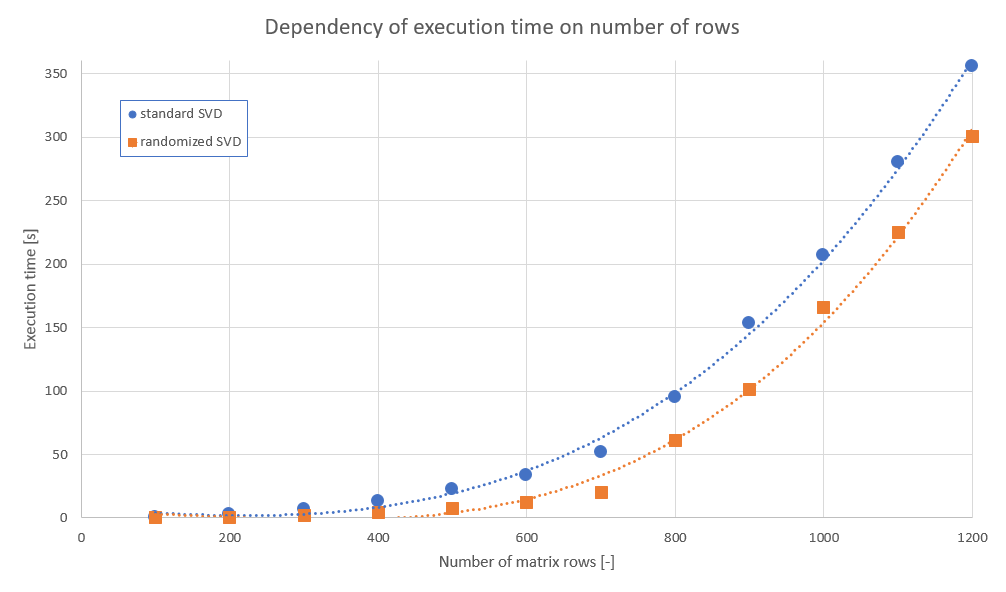
\includegraphics[width=\textwidth]{figures/chapter-SVD/executionTime_varyingRows}
\decoRule
\caption[Dependency of SVD execution time on number of rows.]{Dependency of SVD execution time on $m$ (having fixed $n = 10000$ and $r=min(m,n)$).}
\label{fig:ExeTime_rows}
\end{figure}

\begin{figure}[H]
\centering
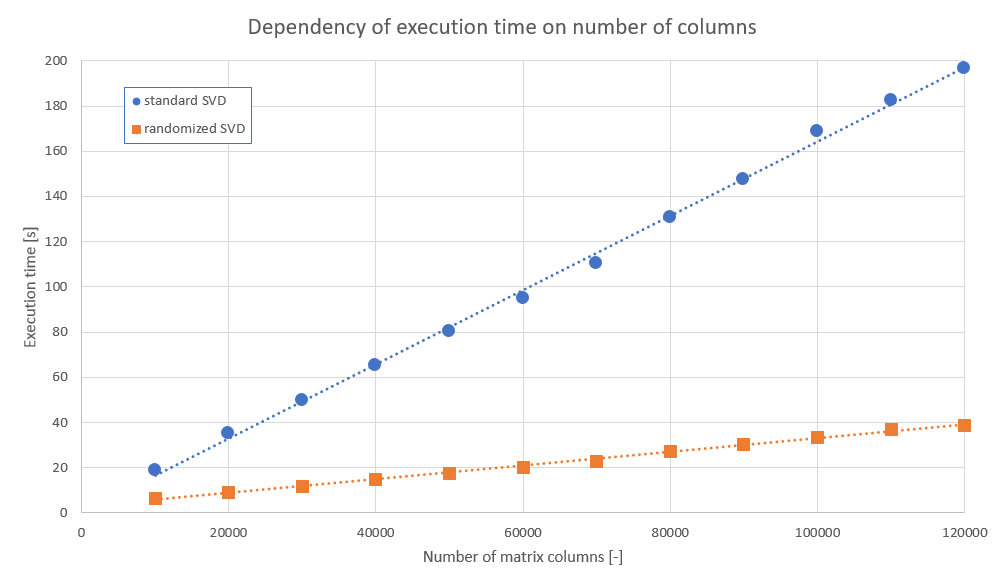
\includegraphics[width=\textwidth]{figures/chapter-SVD/executionTime_varyingColumns}
\decoRule
\caption[Dependency of SVD execution time on number of columns.]{Dependency of SVD execution time on $n$ (having fixed $m = 100$ and $r=min(m,n)$).}
\label{fig:ExeTime_columns}
\end{figure}

% reactor containment
Behavior of the compression strategy introduced is presented on three real world examples. First example is an analysis of aging of nuclear power plant's containment made from prestressed concrete. The finite element mesh used in this analysis is in Figure \ref{fig:temelin:mesh}. More details about the analysis can be found in \cite{Kruis2012} and \cite{Koudelka2009}. This analysis includes high number of analysis time steps (thousands) with very little differences between them. There is therefore potential for compression to be very effective (compression ratio to be very low) as proven in Figure \ref{fig:temelin:NRMSD} that examines the impact of changes in the compression ratio to the mean error of approximation.

\begin{figure}[H]
\centering
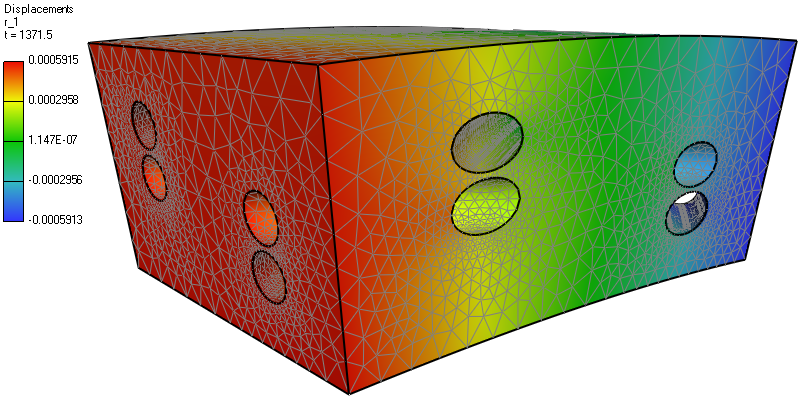
\includegraphics[width=\textwidth]{figures/chapter-SVD/temelin_screenshot}
\decoRule
\caption[Results visualization: reactor containment 3D.]{Segment of reactor containment analyzed. Results visualization (displacement field, x component).}
\label{fig:temelin:mesh}
\end{figure}

\begin{figure}[H]
\centering
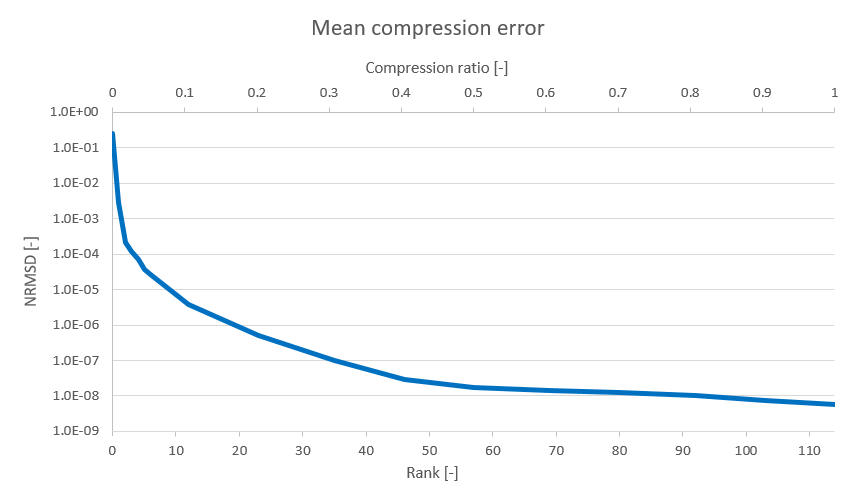
\includegraphics[width=\textwidth]{figures/chapter-SVD/temelin_NRMSD}
\decoRule
\caption[Dependence of NRMSD on compression ratio and rank (reactor containment 3D).]{Dependence of $\mathit{NRMSD}$ on $c$ and $r$ for reactor containment analysis results.} % ...$c$ (and $r$)...
\label{fig:temelin:NRMSD}
\end{figure}

% geological layers
Figure \ref{fig:chotkova:mesh} shows results from an analysis of geological layers which was based on theory of plasticity. More details can be found in \cite{Koudelka2006}. This project was chosen mainly to study behavior of compression algorithm when dealing with high discontinuities in data in spatial dimension (as can be seen in visualization). As summarized in Figure \ref{fig:chotkova:NRMSD} and Figure \ref{fig:chotkova:MaxError} this has negligible effect ($\mathit{NRMSD}$ and $\mathit{NME}$ are bellow 1\% even for very small $r$ -- 3 out of 22) on quality of compression.

\begin{figure}[H]
\centering
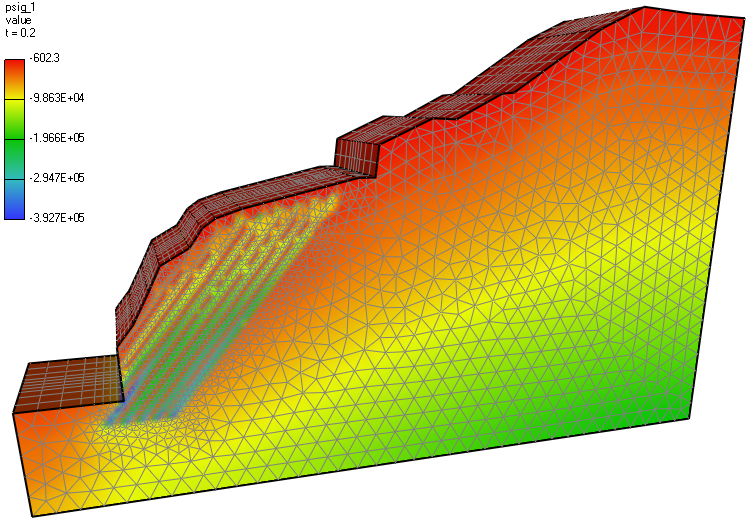
\includegraphics[width=\textwidth]{figures/chapter-SVD/chotkova_screenshot}
\decoRule
\caption[Results visualization: geological layers.]{Analysis of geological layers. Results visualization (stress field, sigma XX component).}
\label{fig:chotkova:mesh}
\end{figure}

\begin{figure}[H]
\centering
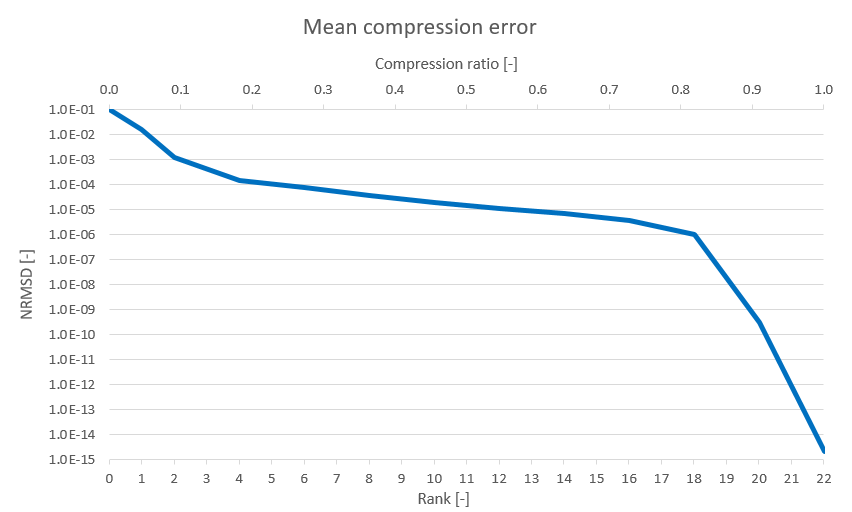
\includegraphics[width=\textwidth]{figures/chapter-SVD/chotkova_NRMSD}
\decoRule
\caption[Dependence of NRMSD on compression ratio and rank (geological layers).]{Dependence of $\mathit{NRMSD}$ on $c$ and $r$ for results of geological layers project.}
\label{fig:chotkova:NRMSD}
\end{figure}

\begin{figure}[H]
\centering
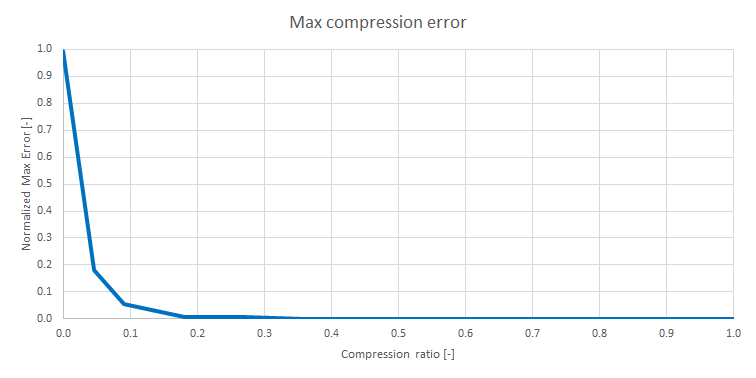
\includegraphics[width=\textwidth]{figures/chapter-SVD/chotkova_MaxError}
\decoRule
\caption[Dependence of NME on compression ratio and rank (geological layers).]{Dependence of $\mathit{NME}$ on $c$ and $r$ for results of geological layers project.}
\label{fig:chotkova:MaxError}
\end{figure}

% reactor vessel 2D
Figure \ref{fig:mechaxisym:mesh} contains visualization of results of two-dimensional analysis, where axisymmetric description was used for analysis of aging of a reactor vessel. Details about the analysis can be found in \cite{Kruis2005}. There are exactly 232 analysis time steps. The resulting data has linear function character with several discontinuities in temporal dimension. There are few time steps in which resulting discrete functions have very different values compared to neighboring time steps. This was supposed to have negative impact on the quality of compression. However, as can be seen in Figure \ref{fig:mechaxisym:NRMSD}, the quality is better than expected; e.g., if the rank of approximation matrix is set to 3 (compared to 232 being the rank of the original matrix) the normalized relative error ($\mathit{NRMSD}$) does not exceed $10^{-5}$.

\begin{figure}[H]
\centering
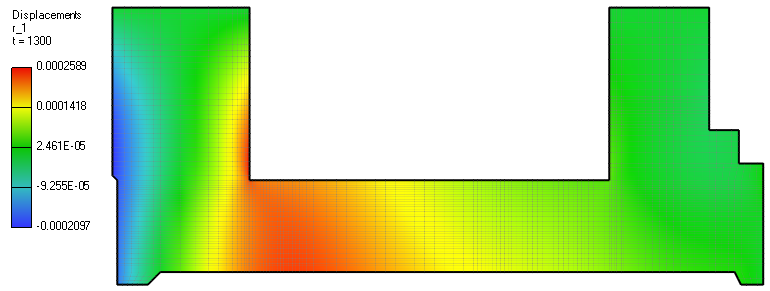
\includegraphics[width=\textwidth]{figures/chapter-SVD/mechaxisym_screenshot}
\decoRule
\caption[Results visualization: reactor vessel 2D.]{2D model of a reactor vessel. Results visualization (displacement field, x component).}
\label{fig:mechaxisym:mesh}
\end{figure}

\begin{figure}[H]
\centering
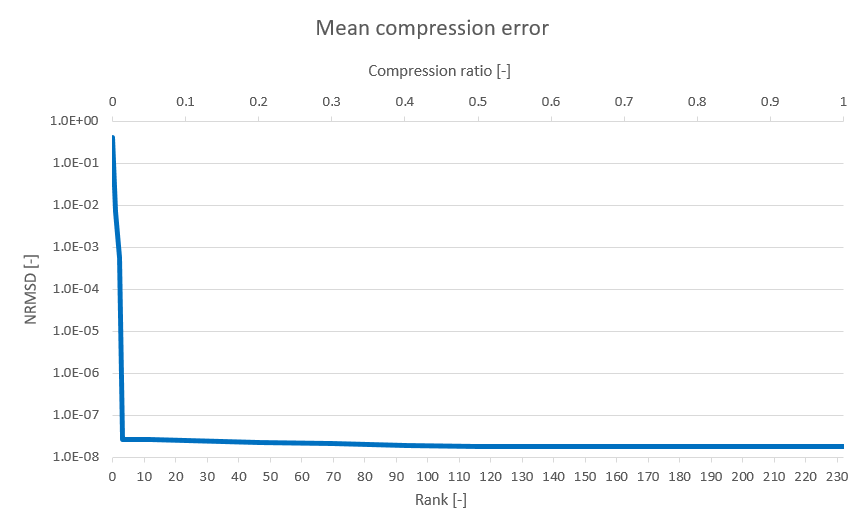
\includegraphics[width=\textwidth]{figures/chapter-SVD/mechaxisym_NRMSD}
\decoRule
\caption[Dependence of NRMSD on compression ratio and rank (reactor vessel 2D).]{Dependence of $\mathit{NRMSD}$ on $c$ and $r$ for reactor vessel analysis results.}
\label{fig:mechaxisym:NRMSD}
\end{figure}

% PSNR
Figure \ref{fig:PSNR} summarizes the compression error for all three benchmarks using $\mathit{PSNR}$ metric. $\mathit{PSNR}$ is defined using logarithm (see Equation (\ref{eq:psnr-def}) for definition), and is included here mainly as a comparison to other image-related compression methods whose quality is often expressed by $\mathit{PSNR}$. Figure \ref{fig:PSNR_rand} contains the same information for the randomized SVD algorithm.

\begin{figure}[H]
\centering
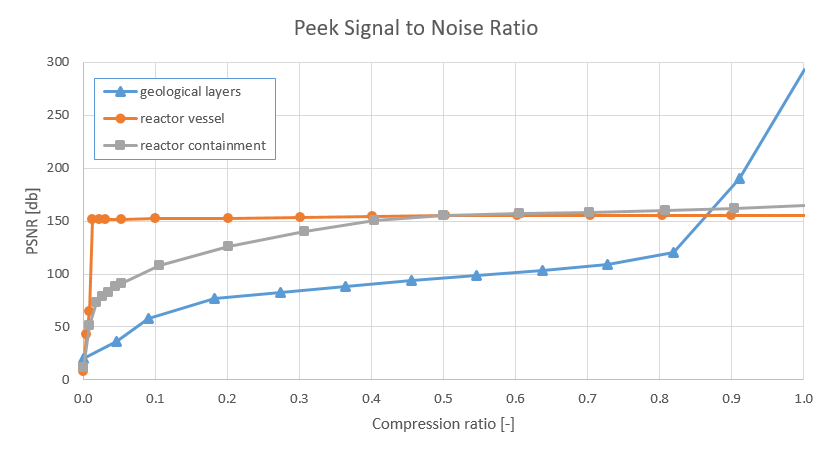
\includegraphics[width=\textwidth]{figures/chapter-SVD/PSNR}
\decoRule
\caption[Dependence of PSNR on compression ratio and rank.]{Dependence of $\mathit{PSNR}$ value on $c$ and $r$ calculated for different SVD decompositions.}
\label{fig:PSNR}
\end{figure}

\begin{figure}[H]
\centering
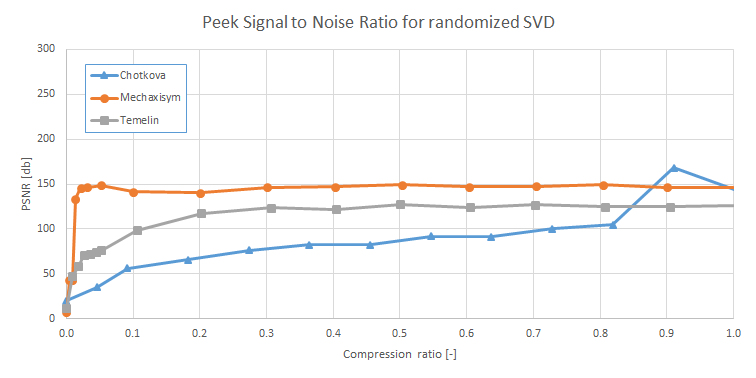
\includegraphics[width=\textwidth]{figures/chapter-SVD/PSNR_rand}
\decoRule
\caption[Dependence of PSNR on compression ratio and rank (randomized SVD).]{Dependence of $\mathit{PSNR}$ value on $c$ and $r$ calculated for different randomized SVD decompositions.}
\label{fig:PSNR_rand}
\end{figure}

% Execution times
Besides the error also the execution speed of compression algorithm was measured. In Figure \ref{fig:temelin:ExeTime}, there is a comparison of execution times for standard versus randomized SVD compression algorithms. Interestingly, execution time of standard SVD is independent of target rank whereas execution time of randomized SVD decreases linearly with decreasing target rank. If the rank is known ahead, the fact can be taken advantage of.

\begin{figure}[H]
\centering
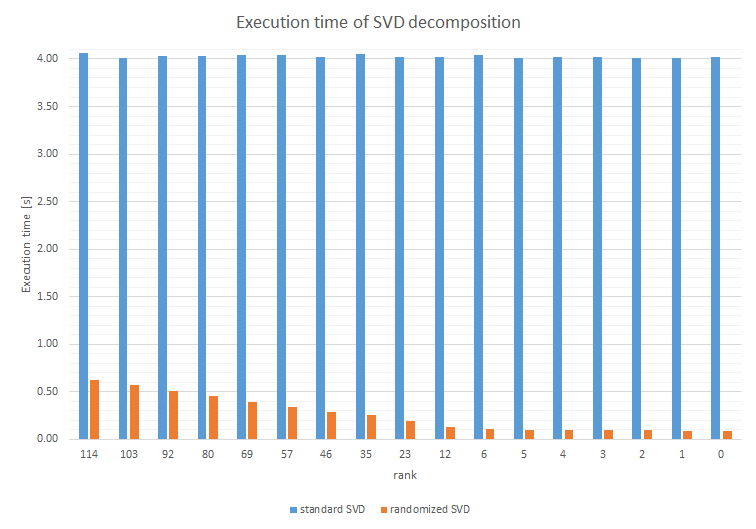
\includegraphics[width=\textwidth]{figures/chapter-SVD/temelin_ExecutionTime}
\decoRule
\caption[Execution time of standard and randomized SVD decompositions.]{Variation of execution time of standard and randomized SVD decompositions calculated for reactor containment analysis results.}
\label{fig:temelin:ExeTime}
\end{figure}

The memory consumption of compressed results for reactor containment analysis is summarized in Table \ref{tab:mem-consum}. For different values of compression ratio it shows memory size in megabytes. In this benchmark, the compression ratio $c$ is an input parameter to the compression algorithm. As follows from the Equation (\ref{eq:rank-from-comp-ratio}), the value of the compression ratio directly affects the amount of singular values ought to be removed from SVD. Size factor describes the final outcome of compression when compared to the original size.

\begin{table}[H]
\caption{Memory consumption of compressed results. 3D reactor containment analysis.}
\label{tab:mem-consum}
\centering
\begin{tabular}{| r | r | r |}
\hline
\tabhead{compression ratio (\textit{\textbf{c}})} & \tabhead{memory consumption [MB]} & \tabhead{size factor} \\
\hline
1.00 & 2002.1 & 1 \\
0.50 & 1006.9 & 0.5002 \\
0.10& 211.9 & 0.1053 \\
0.01 & 35.3 & 0.0176 \\
\hline
\end{tabular}
\end{table}
